\documentclass{beamer}
%
% Choose how your presentation looks.
%
% For more themes, color themes and font themes, see:
% http://deic.uab.es/~iblanes/beamer_gallery/index_by_theme.html
%
\mode<presentation>
{
  \usetheme{Darmstadt}      % or try Darmstadt, Madrid, Warsaw, ...
  \usecolortheme{default}
  \usepackage{beamerthemesplit}% or try albatross, beaver, crane, ...
  \usefonttheme{default}  % or try serif, structurebold, ...
  \setbeamertemplate{navigation symbols}{}
  \setbeamertemplate{caption}[numbered]
} 

\usepackage[english]{babel}
\usepackage[utf8x]{inputenc}
\usepackage{amsmath}
\usepackage{algorithm,algpseudocode}
\usepackage{hyperref}
\hypersetup{
    filecolor=magenta,      
    urlcolor=cyan,
}

\logo{
\includegraphics[height=0.75cm]{images/logo.jpg}}
\title[Support Vector Machine \hspace{0.5cm}\insertframenumber/\inserttotalframenumber]{Support Vector Machine}
\author{Wenfeng Luo}
\institute{Sun Yat-sen University}
\date{12-22-2018}

\begin{document}

\begin{frame}
  \titlepage
\end{frame}

\begin{frame}{Margins: Intuition}

\begin{itemize}
    \item Functional Margin
    \item Logistic Regression $P(y=1|x;\theta) = \sigma(\theta^Tx)$.
    \item If $\sigma(\theta^Tx) > 0.5$, predict $y=1$; otherwise, $y=0$.
    \item The larger $\theta^Tx$ is, the more confident our degree of "confidence" that the label is 1.
\end{itemize}

    
\end{frame}

\begin{frame}{Margins: Intuition}
\begin{itemize}
    \item Geometric Margin
    \item Point A: far away from the decision boundary, we're very confident that A belongs to class $\times$.
    \item Point C: very close to the decision boundary, small changes to the separating hyper-plane will cause out C's prediction to be class $\circ$
    \item Point B: in-between case
    \item We want a decision boundary yielding \textbf{correct} and \textbf{confident} predictions.
    \begin{figure}
    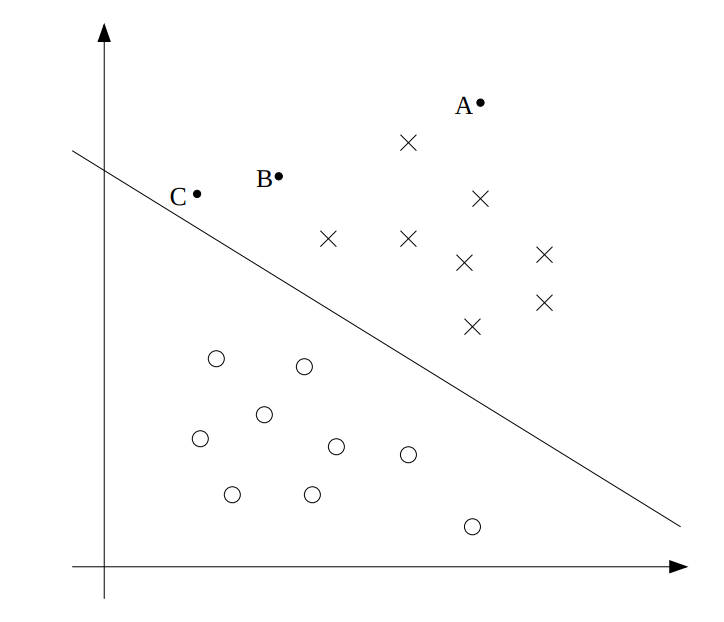
\includegraphics[width=4cm]{images/img1.png}
    \end{figure}
\end{itemize}    
\end{frame}

% Uncomment these lines for an automatically generated outline.
%\begin{frame}{Outline}
%  \tableofcontents
%\end{frame}
%\section{Introduction}

\begin{frame}{Notation}
\begin{itemize}
\item features: $x \in \mathbb{R}^n$
\item labels: $y\in \{-1, 1\}$
\item training data: $\{(x^{(1)}, y^{(1)}),(x^{(2)}, y^{(2)}),...,(x^{(m)}, y^{(m)})\}$
\item parameters: $w, b$
\item classifier:
\begin{align}
\begin{split}
h_{w, b}(x) &= g(w^Tx + b)\\
g(z) &=
  \begin{cases}
    1       & z > 0\\
    -1  & z < 0
  \end{cases}
\end{split}
\end{align}

\end{itemize}
\end{frame}

\begin{frame}{Geometric Margin}
\begin{figure}
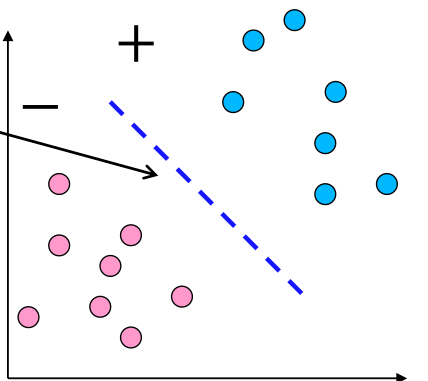
\includegraphics[width=4cm]{images/img3.png}
\end{figure}
\begin{itemize}
\item Decision boundary
\begin{equation}
w^Tx + b = 0
\end{equation}
\item Classifier $f(x) = \text{sign}(w^Tx+b)$
\end{itemize}
\end{frame}

\begin{frame}{Maximal Margin}
\begin{figure}
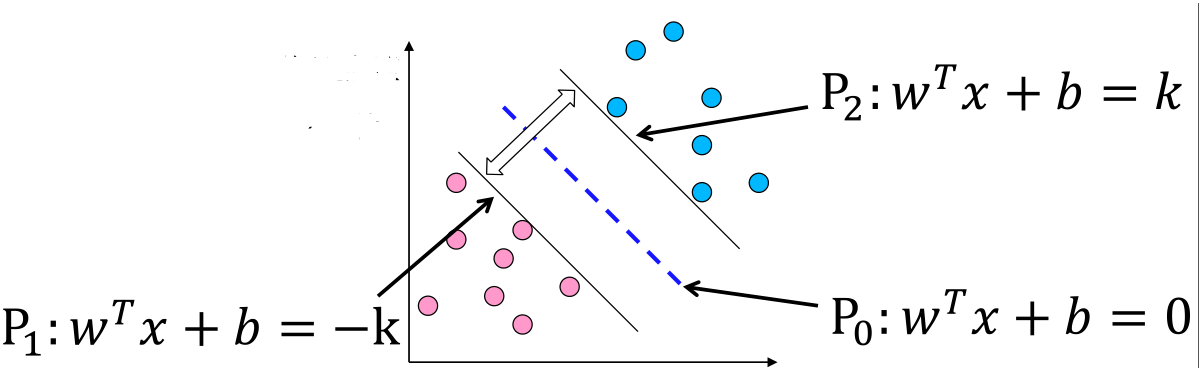
\includegraphics[width=8cm]{images/img4.png}
\end{figure}
\begin{itemize}
\item Distance between P1 and P2
\begin{equation}
\text{margin} = \frac{k-(-k)}{\sqrt{w_1^2+...+w_n^2}}=\frac{2k}{||w||_2}
\end{equation}
\item Our goal is to maximize the margin.
\end{itemize}
\end{frame}

\begin{frame}{Optimization Problem}
\begin{itemize}
\item  Optimization Problem 0
\begin{align}
\begin{split}
\text{argmax}_{w, b}\text{   }&\frac{2k}{||w||_2} \\
\text{s.t.} \text{   }&w^Tx^{(i)} + b \geq k, \text{for } y^{(i)} = 1\\
\text{   }&w^Tx^{(i)} + b \leq -k, \text{for } y^{(i)} = -1 \\
\end{split}
\end{align}
\item  Optimization Problem 1
\begin{align}
\begin{split}
\text{argmax}_{w, b}\text{   }&\frac{2k}{||w||_2} \\
\text{s.t.} \text{   }&y^{(i)}(w^Tx^{(i)} + b) \geq k
\end{split}
\end{align}
\end{itemize}
\end{frame}

\begin{frame}{Optimization Problem}
\begin{itemize}
\item  Optimization Problem 2
\begin{align}
\begin{split}
\text{argmax}_{w, b}\text{   }&\frac{2}{||\frac{w}{k}||_2} \\
\text{s.t.} \text{   }&y^{(i)}\left(\left(\frac{w}{k}\right)^Tx^{(i)} + \frac{b}{k}\right) \geq 1
\end{split}
\end{align}
\item  Optimization Problem 3($w' = \frac{w}{k}, b'=\frac{b}{k}$)
\begin{align}
\begin{split}
\text{argmax}_{w', b'}\text{   }&\frac{2}{||w'||_2} \\
\text{s.t.} \text{   }&y^{(i)}\left(w'^Tx^{(i)} + b'\right) \geq 1
\end{split}
\end{align}
\end{itemize}
\end{frame}

\begin{frame}{Optimization Problem}
\begin{itemize}
\item  Optimization Problem 4
\begin{align}
\begin{split}
\text{argmax}_{w, b}\text{   }&\frac{2}{||w||_2} \\
\text{s.t.} \text{   }&y^{(i)}\left(w^Tx^{(i)} + b\right) \geq 1
\end{split}
\end{align}
\item  Optimization Problem 5
\begin{align}
\begin{split}
\text{argmin}_{w, b}\text{   }&\frac{1}{2}||w||_2 \\
\text{s.t.} \text{   }&y^{(i)}\left(w^Tx^{(i)} + b\right) \geq 1
\end{split}
\end{align}
\end{itemize}
\end{frame}

\begin{frame}{Optimization Problem}
\begin{align}
\begin{split}
\text{argmin}_{w, b}\text{   }&\frac{1}{2}w^Tw \\
\text{s.t.} \text{   }&y^{(i)}\left(w^Tx^{(i)} + b\right) \geq 1\\
&i = 1,...,m
\end{split}
\end{align}
\begin{itemize}
\item Convex optimization problem
\item Okay if the data is linearly separable
\end{itemize}
\end{frame}

\begin{frame}{What are the Support Vectors?}
\begin{figure}
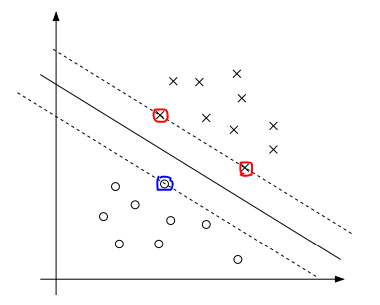
\includegraphics[width=4cm]{images/img5.png}
\end{figure}
\begin{itemize}
\item Support Vectors are those data points that are closest to the decision boundary
\item Number of support vectors could be much smaller than the size of the training set
\end{itemize}
\end{frame}

\begin{frame}{Regularization and the non-separable case}
\begin{itemize}
\item What if the data is not linearly separable?
\item How to deal with outliers?
\begin{tabular}{cc}

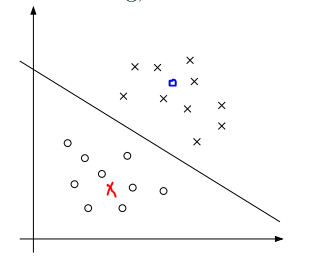
\includegraphics[width=4cm]{images/img6.png}
& 
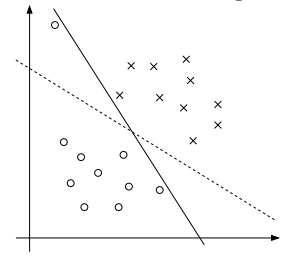
\includegraphics[width=4cm]{images/img7.png} \\

(a) Linearly non-separable & (b) Outliers\\
\end{tabular}
\end{itemize}
\end{frame}

\begin{frame}{Regularization and the non-separable case}
\begin{align}
\begin{split}
\text{argmin}_{w, b}\text{   }&\frac{1}{2}w^Tw \\
\text{s.t.} \text{   }&y^{(i)}\left(w^Tx^{(i)} + b\right) \geq 1\\
&i = 1,...,m
\end{split}
\end{align}
\begin{itemize}
\item Allow the constrain of some data points not strictly satisfied
\item And add in a penalization term($l_1$ norm)
\item Optimization problem 6
\begin{align}
\begin{split}
\text{argmin}_{w, b, \xi}\text{   }&\frac{1}{2}w^Tw + C\sum_i^m \xi_i  \\
\text{s.t.} \text{   }&y^{(i)}\left(w^Tx^{(i)} + b\right) \geq 1-\xi_i, i = 1,...,m\\
&\xi_i \geq 0, i = 1,...,m\\
\end{split}
\end{align}
\end{itemize}
\end{frame}

\begin{frame}{Optimization Problem}
\begin{align}
\begin{split}
\text{argmin}_{w, b, \xi}\text{   }&\frac{1}{2}w^Tw + C\mathbf{1}^T\xi  \\
\text{s.t.} \text{   }&y^{(i)}\left(w^Tx^{(i)} + b\right) \geq 1-\xi_i, i = 1,...,m\\
&\xi_i \geq 0, i = 1,...,m\\
\end{split}
\end{align}
\begin{itemize}
\item C is a constant, just like the regularization hyper-parameter.
\item How to find the optimal solution?
\item \textbf{Lagrange multiplier} and \textbf{Coordinate descent}.
\end{itemize}
\end{frame}

\begin{frame}{Lagrange duality}
\begin{itemize}
\item Consider the problem
\begin{align*}
\begin{split}
\min_w\text{ }&f(w) \\
\text{s.t. }&h_i(w) = 0, i=1,...,m\\
\end{split}
\end{align*}
\item Define \textbf{Lagrangian} to be
\begin{align*}
\mathcal{L}(w, \beta) &= f(w) + \sum_i^m \beta_i h_i(w) \\
\end{align*}
\item $\beta_i$'s are the Lagrange multipliers
\item Compute the partial derivative and set them to 0
\begin{align*}
  \begin{cases}
    \frac{\partial\mathcal{L}}{\partial w} = 0\\
    \frac{\partial\mathcal{L}}{\partial \beta_i} = 0, i=1,...,m
  \end{cases}
\end{align*}
\end{itemize}
\end{frame}

\begin{frame}{Lagrange duality}
\begin{itemize}
\item More generally, there are both equality and inequality constrains
\item Consider the following optimization problem
\begin{align*}
\begin{split}
\min_w\text{ }&f(w) \\
\text{s.t. } &g_i(w) \leq 0, i=1,..,k\\
\text{s.t. } &h_i(w) = 0, i=1,..,l\\
\end{split}
\end{align*}
\item Define the \textbf{generalized Lagrangian}
\begin{align*}
\mathcal{L}(w, \alpha, \beta) &= f(w) + \sum_{i=1}^k\alpha_ig_i(w) + \sum_{i=1}^l\beta_ih_i(w) \\
\alpha_i&\geq0,i=1,...,m \\
\max_{\alpha, \beta} \mathcal{L} &= \begin{cases}
f(w) & \text{constrain satisfied}\\
\infty & \text{otherwise}
\end{cases}
\end{align*}
\end{itemize}
\end{frame}

\begin{frame}{Lagrange Duality}
\begin{itemize}
\item \textbf{Primal} Problem 
\begin{align*}
	\min_x\max_{\alpha, \beta} \mathcal{L}
\end{align*}
\item \textbf{Dual} Problem 
\begin{align*}
	\max_{\alpha, \beta}\min_x \mathcal{L}
\end{align*}
\item This two problems are equal
\end{itemize}
\begin{align}
\min_x\max_{\alpha, \beta} \mathcal{L} = \max_{\alpha, \beta}\min_x \mathcal{L}
\end{align}
\end{frame}


\begin{frame}{Saddle-point Interpretation}
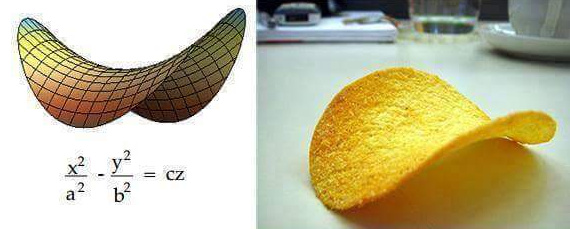
\includegraphics[width=\textwidth]{images/saddle.png}
\end{frame}

\begin{frame}{Optimization Problem}
\begin{itemize}
\item Optimization Problem 5
\begin{align}
\begin{split}
\text{argmin}_{w, b, \xi}\text{   }&\frac{1}{2}w^Tw + C\sum_{i=1}^m\xi_i \\
\text{s.t.} \text{   }&y^{(i)}\left(w^Tx^{(i)} + b\right) \geq 1-\xi_i, i = 1,...,m\\
&\xi_i\geq0, i=1,...,m\\
\end{split}
\end{align}
\item Optimization Problem 6
\begin{align}
\begin{split}
\text{argmax}_{\alpha}\text{   }&\sum_{i=1}^m\alpha_i - \frac{1}{2}\sum_{i,j=1}^my^{(i)}y^{(j)}\alpha_i\alpha_j\langle x^{(i)}, x^{(j)}\rangle \\
\text{s.t.} \text{   }&0\leq \alpha_i \leq C, i=1,...,m\\
&\sum_{i=1}^m\alpha_iy^{(i)}=0
\end{split}
\end{align}
\end{itemize}
\end{frame}

\begin{frame}{Optimization Problem 5 $\to$ 6}
\begin{itemize}
	\item Constrain $y^{(i)}\left(w^Tx^{(i)} + b\right) \geq 1-\xi_i$ and $\xi_i\geq0$
	\item Constrain $-(y^{(i)}\left(w^Tx^{(i)} + b\right)-1+\xi_i) \leq 0$ and $-\xi_i\leq0$
\begin{align*}
L(w, b, \xi) &= \frac{1}{2}w^Tw + C\sum_{i=1}^m\xi_i\\
&-\sum_{i=1}^m\alpha_i\left(y^{(i)}(w^Tx^{(i)} +b) - 1 + \xi_i\right) - \sum_{i=1}^m\beta_i\xi_i\\
\frac{\partial L}{\partial w} &= w - \sum_{i=1}^m\alpha_iy^{(i)}x^{(i)}\\
\frac{\partial L}{\partial b} &= -\sum_{i=1}^m\alpha_iy^{(i)}\\
\frac{\partial L}{\partial \xi_i} &= C-\alpha_i-\beta_i\\
\end{align*}
\end{itemize}
\end{frame}

\begin{frame}{Optimization Problem 5 $\to$ 6}
\begin{align}
\frac{\partial L}{\partial w}&=0\to w = \sum_{i=1}^m\alpha_iy^{(i)}x^{(i)}\\
\frac{\partial L}{\partial b}&=0\to\sum_{i=1}^m\alpha_iy^{(i)}=0\\
\frac{\partial L}{\partial \xi_i}&=0\to\beta_i= C-\alpha_i(0\leq\alpha_i\leq C)
\end{align}
\end{frame}

\begin{frame}{Optimization Problem 5 $\to$ 6}
\begin{itemize}
\item Use $w = \sum_{i=1}^m\alpha_iy^{(i)}x^{(i)}, \beta_i= C-\alpha_i$, substitude back to $\mathcal{L}$
\end{itemize}
\begin{align*}
\begin{split}
L(w, b, \xi) =& \frac{1}{2}w^Tw -\sum_{i=1}^m\alpha_iy^{(i)}w^Tx^{(i)}-b\sum_{i=1}^m\alpha_iy^{(i)}+\\ &(C-\alpha_i-\beta_i)\sum_{i=1}^m\xi_i+\sum_{i=1}^m\alpha_i\\
=&\frac{1}{2}\left(\sum_{i=1}^m\alpha_iy^{(i)}x^{(i)}\right)^T\left(\sum_{i=1}^m\alpha_iy^{(i)}x^{(i)}\right)-\\
&\sum_{i=1}^m\alpha_iy^{(i)}\left(\sum_{j=1}^m\alpha_iy^{(j)}x^{(j)}\right)^Tx^{(i)} +\sum_{i=1}^m\alpha_i\\
=&\sum_{i=1}^m\alpha_i-\frac{1}{2}\sum_{i,j=1}^m\alpha_i\alpha_jy^{(i)}y^{(j)}\langle x^{(i)}, x^{(j)}\rangle
\end{split}
\end{align*}
\end{frame}

\begin{frame}{Optimization Problem 6}

\begin{align*}
\begin{split}
\text{argmax}_{\alpha}\text{   }&\sum_{i=1}^m\alpha_i - \frac{1}{2}\sum_{i,j=1}^my^{(i)}y^{(j)}\alpha_i\alpha_j\langle x^{(i)}, x^{(j)}\rangle \\
\text{s.t.} \text{   }&0\leq \alpha_i \leq C, i=1,...,m\\
&\sum_{i=1}^m\alpha_iy^{(i)}=0
\end{split}
\end{align*}
\begin{itemize}
	\item The Primal problem still belongs to semi-programming, no better than optimization 5
	\item Only inner product of input feature matters
\end{itemize}
\end{frame}

\begin{frame}{KKT Conditions}
\begin{itemize}
	\item $\alpha_i=0, y^{(i)}(w^Tx^{(i)}+b)\geq 1$: $x^{(i)}$, outside the margin;
	\item $0< \alpha< C, y^{(i)}(w^Tx^{(i)}+b) = 1$: $x^{(i)}$ on the margin;
	\item $\alpha_i=C, y^{(i)}(w^Tx^{(i)}+b) \leq 1$: $x^{(i)}$ inside margin.
	\item After optimizing over $\alpha$'s, recover the original model parameter $w, b$
	\begin{align}\label{eq:wb}
	\begin{split}
	w=&\sum_{i=1}^m\alpha_iy^{(i)}x^{(i)}\\
	b=&-\frac{1}{2}\left(\min_{y^{(i)}=1}w^Tx^{(i)} + \max_{y^{(i)}=-1}w^Tx^{(i)}\right)
	\end{split}
	\end{align}
	\item A new data point $x$
	\begin{align*}
		w^Tx + b = \sum_{i=1}^m\alpha_iy^{(i)}\langle x^{(i)}, x\rangle + b =\sum_{i\in S}\alpha_iy^{(i)}\langle x^{(i)}, x\rangle + b
	\end{align*}
\end{itemize}
\end{frame}

\begin{frame}{Kernel Trick}
\begin{itemize}
\item Feature mapping $\phi$, say
\begin{align*}
\phi(x) = \begin{bmatrix}
x\\
x^2\\
x^3
\end{bmatrix}
\end{align*}
\item For specific mapping $\phi$, define the corresponding \textbf{Kernel} to be
\begin{align*}
K(x^{(i)}, x^{(j)}) = \langle \phi(x^{(i)}), \phi(x^{(j)})\rangle
\end{align*}
\item We want to use the feature $\phi(x)$, non-linearity
\item Simply replace $\langle x^{(i)}, x^{(j)}\rangle$ with $K(x^{(i)}, x^{(j)})$
\item Interestingly, $K(x^{(i)}, x^{(j)})$ could be efficiently computed without having to go through the actual feature mapping $\phi(x)$.
\end{itemize}
\end{frame}

\begin{frame}{Kernel Trick}
\begin{itemize}
	\item Compute $K(x, z) = (x^Tz)^2$, $O(n)$
	\item Write $K(x, z)$ differently
	\begin{align*}
		K(x, z) & = \left(\sum_{i=1}^mx_iz_i\right)^T\left(\sum_{i=1}^mx_iz_i\right)\\
		& = \sum_{i=1}^m\sum_{j=1}^mx_ix_jz_iz_j\\
		&=\sum_{i,j=1}^m(x_ix_j)(z_iz_j)
	\end{align*}
\end{itemize}
\end{frame}

\begin{frame}{Kernel Trick}
\begin{itemize}
	\item Compute $K(x, z) = (x^Tz)^2$, $O(n)$
	\item Write $K(x, z)$ differently $K(x, z)=\sum_{i,j=1}^m(x_ix_j)(z_iz_j)$
	\item The corresponding feature mapping is
	\begin{align*}
		\phi(x) = \begin{bmatrix}
		x_1x_1\\
		x_1x_2\\
		x_1x_3\\
		x_2x_1\\
		x_2x_2\\
		x_2x_3\\
		x_3x_1\\
		x_3x_2\\
		x_3x_3
		\end{bmatrix}
	\end{align*}
	\item Compute $K(x, z) = \phi(x)^T\phi(z)$, $O(n^2)$
\end{itemize}
\end{frame}

\begin{frame}
\begin{itemize}
	\item A related kernel
	\begin{align*}
	K(x, z) &= (x^Tz+c)^2=\sum_{i,j=1}^n(x_ix_j)(z_iz_j) + \sum_{i=1}^n(\sqrt{2c}x_i)(\sqrt{2c}z_i) + c^2
	\end{align*}
	\item The corresponding feature mapping is
	\begin{align*}
	\phi(x) = \begin{bmatrix}
	x_1x_1\\
	x_1x_2\\
	x_1x_3\\
	x_2x_1\\
	x_2x_2\\
	x_2x_3\\
	x_3x_1\\
	x_3x_2\\
	x_3x_3\\
	\sqrt{2c}x_1\\
	\sqrt{2c}x_2\\
	\sqrt{2c}x_3\\
	c
	\end{bmatrix}
	\end{align*}
\end{itemize}
\end{frame}

\begin{frame}{Common Kernel Functions}
\begin{itemize}
	\item Linear kernel $K(x, z) = x^Tz$
	\item Polynomial Kernel $K(x, z) = (x^Tz + c)^d$
	\item Gaussian Kernel (RBF) $K(x, z) = \exp\{-\frac{||x - z||^2}{2\sigma^2}\}$, infinite dimension.
	\item Sigmoid, ...
	\item The point is if you could prove there exists a feature mapping $\phi(x)$ such that $K(x, z) = \phi(x)^T\phi(z)$, then it's a valid kernel.
\end{itemize}
\end{frame}

\begin{frame}{Kernel Trick}
We only need the output $K(x, z)$ and we don't have to go through the procedure 
\begin{align*}
(x, z)\to(\phi(x), \phi(z))\to\phi(x)^T\phi(z)
\end{align*}
\end{frame}

\begin{frame}{Implementation from Sklearn}
\begin{itemize}
\item from sklearn import svm
\end{itemize}
\begin{figure}
	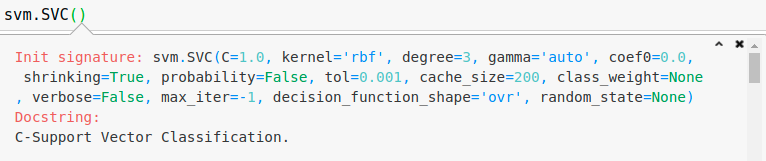
\includegraphics[width=\textwidth]{images/sk_svc.png}
\end{figure}
\end{frame}

\begin{frame}{The SMO algorithm}
\begin{itemize}
\item Coordinate Descent
\end{itemize}
\begin{figure}
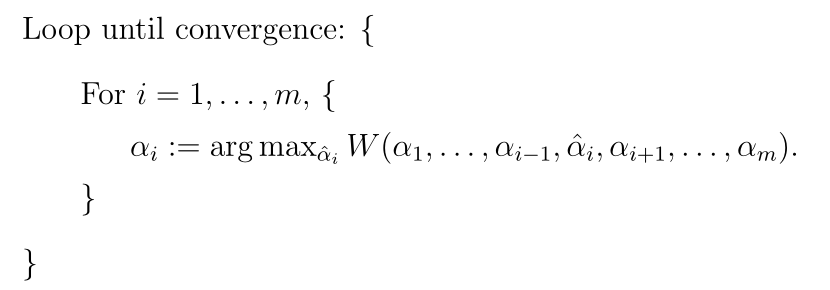
\includegraphics[height=2cm]{images/img9.png}
\end{figure}
\begin{figure}
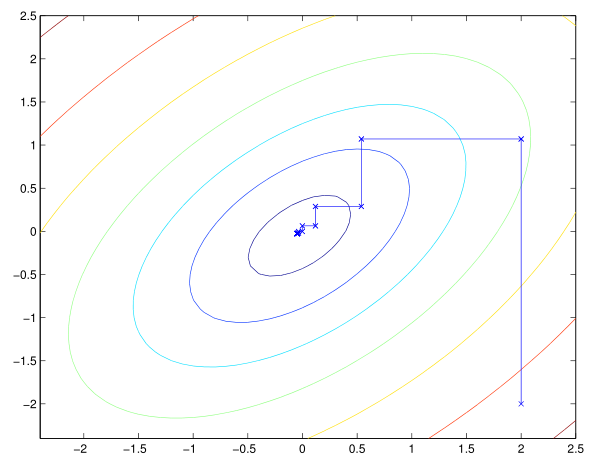
\includegraphics[height=4.6cm]{images/img8.png}
\end{figure}
\end{frame}

\begin{frame}{The SMO algorithm}
\begin{align}
\begin{split}
\text{argmax}_{\alpha}\text{   }&\sum_{i=1}^m\alpha_i - \frac{1}{2}\sum_{i,j=1}^my^{(i)}y^{(j)}\alpha_i\alpha_j\langle x^{(i)}, x^{(j)}\rangle \\
\text{s.t.} \text{   }&0\leq \alpha_i \leq C, i=1,...,m\\
&\sum_{i=1}^m\alpha_iy^{(i)}=0
\end{split}
\end{align}
\begin{itemize}
\item Maximize on $\alpha_1$, fix the other $m-1$ $\alpha$'s?
\begin{equation}
\alpha_1 = -y^{(1)} \sum_{i=2}^m \alpha_iy^{(i)}
\end{equation}
\item If $\alpha_2,...,\alpha_m$ are fixed, then $\alpha_1$ is also a constant, can't do any better.
\end{itemize}
\end{frame}

\begin{frame}{The SMO algorithm}
\begin{align}
\begin{split}
\text{argmax}_{\alpha}\text{   }&\sum_{i=1}^m\alpha_i - \frac{1}{2}\sum_{i,j=1}^my^{(i)}y^{(j)}\alpha_i\alpha_j\langle x^{(i)}, x^{(j)}\rangle \\
\text{s.t.} \text{   }&0\leq \alpha_i \leq C, i=1,...,m\\
&\sum_{i=1}^m\alpha_iy^{(i)}=0
\end{split}
\end{align}
\begin{itemize}
\item Choose two $\alpha$'s, say $\alpha_1, \alpha_2$
\begin{equation}
\alpha_1y^{(1)} + \alpha_2y^{(2)} = -\sum_{i=3}^m\alpha_iy^{(i)}
\end{equation}
\item Denote $\zeta = -\sum_{i=3}^m\alpha_iy^{(i)}$
\begin{equation}
\alpha_1y^{(1)} + \alpha_2y^{(2)} = \zeta
\end{equation}
\end{itemize}
\end{frame}

\begin{frame}{The SMO algorithm}
\begin{align}
\begin{split}
\text{argmax}_{\alpha}\text{   }&\sum_{i=1}^m\alpha_i - \frac{1}{2}\sum_{i,j=1}^my^{(i)}y^{(j)}\alpha_i\alpha_j\langle x^{(i)}, x^{(j)}\rangle \\
\text{s.t.} \text{   }&0\leq \alpha_i \leq C, i=1,...,m\\
&\sum_{i=1}^m\alpha_iy^{(i)}=0
\end{split}
\end{align}
\begin{itemize}
\item $\alpha_1 = y^{(1)}(\zeta - \alpha_2y^{(2)})$
\item Optimization sub-problem(fix $\alpha_3,...,\alpha_m$, replace $\alpha_1$ with $\alpha_2$)
\begin{align}
\begin{split}
\text{argmax}_{\alpha}\text{   }& A\alpha_2^2 + B\alpha_2 \\
\text{s.t.} \text{   }&0\leq \alpha_1, \alpha_2 \leq C\\
\end{split}
\end{align}
\end{itemize}
\end{frame}

\begin{frame}
\begin{figure}
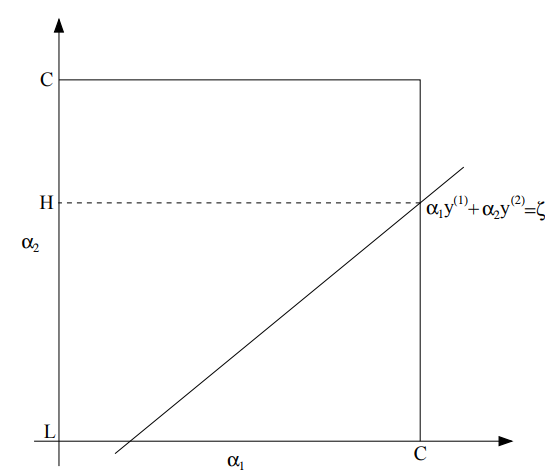
\includegraphics[width=4cm]{images/img14.png}
\end{figure}
\begin{itemize}
\item Both $\alpha_1$ and $\alpha_2$ have to satisfy the box constrain.
\item Consider only the constrain on $L\leq \alpha_2 \leq H$
\item If $y^{(1)}y^{(2)} = 1$
\begin{equation}
\begin{cases}
L = \max(0, \alpha_1^{old}+\alpha_2^{old}-C)\\
H = \min(C, \alpha_1^{old}+\alpha_2^{old})\\
\end{cases}
\end{equation}
\item Else
\begin{equation}
\begin{cases}
L = \max(0, \alpha_2^{old}-\alpha_1^{old})\\
H = \min(C, C+\alpha_2^{old}-\alpha_1^{old})\\
\end{cases}
\end{equation}
\end{itemize}
\end{frame}

\begin{frame}{$y^{(1)}y^{(2)} = 1$}
\begin{itemize}
	\item Both $\alpha_1$ and $\alpha_2$ are in the line
	\begin{align*}
	\alpha_1y^{(1)} + \alpha_2y^{(2)} &=\zeta = \alpha_1^{old}y^{(1)} + \alpha_2^{old}y^{(2)} \\
	\end{align*}
	\item Simply just $\alpha_1 + \alpha_2 =\alpha_1^{old} + \alpha_2^{old}$
	\begin{equation}
	\begin{cases}
	L = \max(0, \alpha_1^{old}+\alpha_2^{old}-C)\\
	H = \min(C, \alpha_1^{old}+\alpha_2^{old})\\
	\end{cases}
	\end{equation}
\end{itemize}
\end{frame}

\begin{frame}
\begin{itemize}
\item $A \sim2\langle x_1, x_2\rangle - \langle x_1, x_1\rangle - \langle x_2, x_2\rangle = -||x_1 - x_2||^2 \leq 0$, so
\end{itemize}
\begin{tabular}{cc}
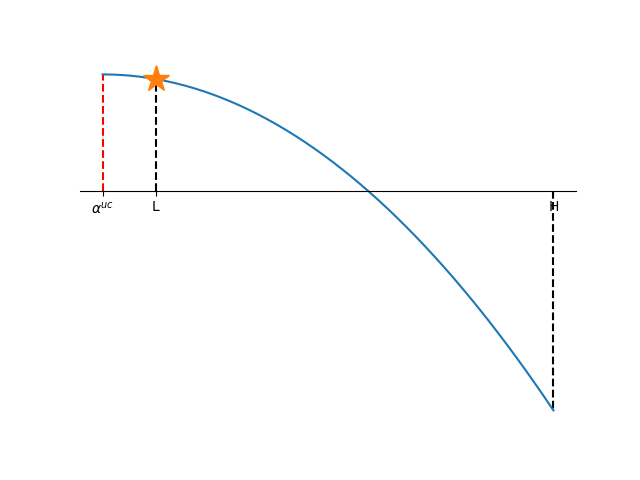
\includegraphics[width=4.5cm]{images/img13.png} & 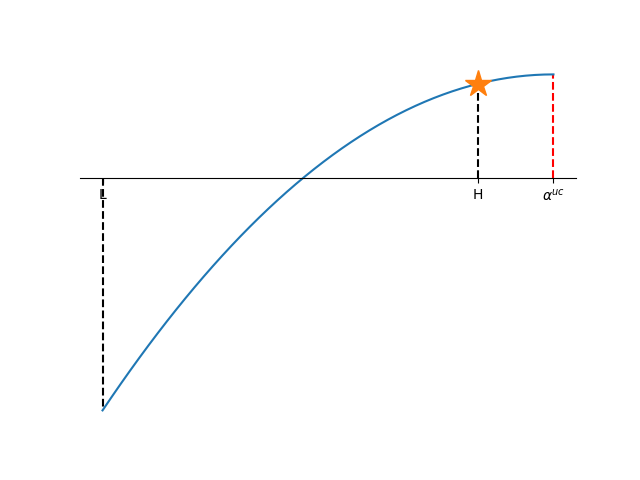
\includegraphics[width=4.5cm]{images/img12.png} \\
(1) $\alpha_2^{uc} < L$ & (2) $\alpha_2^{uc} > H$ \\
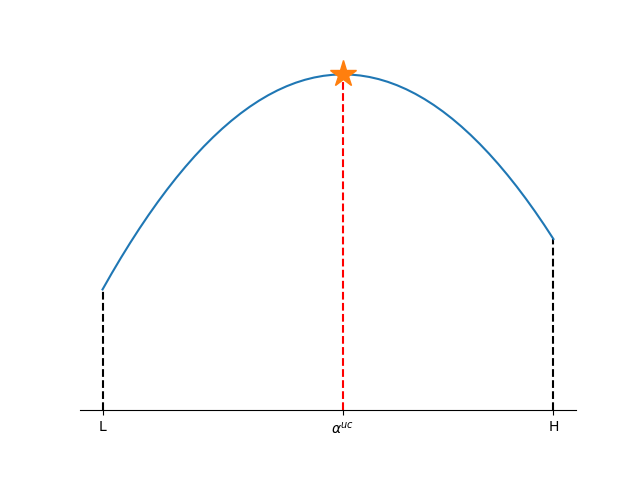
\includegraphics[width=4.5cm]{images/img11.png} &\\
(3) $L \leq \alpha_2^{uc} \leq H$ & \\

\end{tabular}
% import numpy as np
% import matplotlib.pyplot as plt


% def func(x, xh):
%     return -(x - xh)**2 + 1


% xbest = 1.0
% s = -0.0
% L, H = 0.2 - s, 1.7 - s
% xs = np.linspace(min(L, xbest), max(H, xbest))
% ys = func(xs, xbest)
% ax = plt.gca()
% ax.spines['left'].set_visible(False)
% ax.spines['right'].set_visible(False)
% ax.spines['top'].set_visible(False)
% ax.spines['bottom'].set_position('zero')
% ax.yaxis.set_ticks([])
% plt.plot(xs, ys)

% plt.vlines(L, 0.0, func(L, xbest), linestyle='--', color='k')
% plt.vlines(H, 0.0, func(H, xbest), linestyle='--', color='k')
% plt.vlines(xbest, 0.0, func(xbest, xbest), linestyle='--', color='r')
% ax.xaxis.set_ticks([L, H, xbest])
% ax.xaxis.set_ticklabels(['L', 'H', r'$\alpha^{uc}$'])

% a = min(H, max(L, xbest))
% plt.plot([a], [func(a, xbest)], '*', markersize=20)

% plt.show()
\end{frame}

\begin{frame}
\begin{align}
\begin{split}
\text{argmax}_{\alpha_2}\text{   }& A\alpha_2^2 + B\alpha_2 \\
\text{s.t.} \text{   }&L\leq \alpha_2 \leq H\\
\end{split}
\end{align}
\begin{itemize}
\item Denote $\alpha_2^{uc}=-\frac{B}{2A}$, where the superscript stands for "unclipping".
\begin{equation}
\alpha_2^* = \begin{cases}
L, & \alpha_2^{uc} < L \\
H, & \alpha_2^{uc} > H\\
\alpha_2^{uc}, & otherwise\\
\end{cases}
\end{equation}
\item Or put it simple
\begin{align*}
\alpha_2^* &= \min\left(\max\left(L, \alpha_2^{uc}\right), H\right)\\
\alpha_1^* &= y^{(1)}(\zeta - y^{(2)}\alpha_2^*)
\end{align*}
\end{itemize}
\end{frame}

\begin{frame}
\scalebox{0.70}{
\begin{minipage}{\textwidth}
\begin{algorithm}[H] 
	\caption{Simple Implementation of SMO}
	\label{alg:simple_smo}
	\textbf{Input:} $\{(x^{(1)}, y^{(1)}),...(x^{(m)}, y^{(m)})\}$\\
	\textbf{Output:} $w, b$
	\begin{algorithmic}[1]
		\Statex
		\State{Initialize all $\alpha$'s to 0}
		\State{tol=10, iter=0}
		\While{iter $<$ tol}
		\State{iter = iter + 1}
		\For{$i \gets 1$ to $m$}
		\If{KKT condition not satisfied for $\alpha_i$}
		\State{Randomly choose another $\alpha_j$}
		\State{Compute the bound $L$ and $H$ for $\alpha_j$}
		\If{$L = H$}
		\State{\textbf{continue}}
		\EndIf
		\State{iter = 0}
		\State{Compute the unclipping value $\alpha_{j}^{uc}$ for $\alpha_j$}
		\State{$\zeta = \alpha_i^{old}y^{(i)}+\alpha_j^{old}y^{(j)}$}
		\State{$\alpha_j^{new} =  \min(\max(L, \alpha^{uc}_j), H)$}
		\State{$\alpha_i^{new} =  y^{(i)}(\zeta - \alpha_j^{new}y^{(j)})$}
		\EndIf
		\EndFor
		\EndWhile
		\State{Use equation (\ref{eq:wb}) to Compute $w, b$ from $\alpha$'s}
	\end{algorithmic}
\end{algorithm}
\end{minipage}
}
\end{frame}

\begin{frame}{One Possible Implementation}
\begin{itemize}
\item \href{https://github.com/Irlyue/MLAlg/blob/master/code/svm/svm.py}{svm.py}: Kernel functions, SVM class.
\item\href{https://github.com/Irlyue/MLAlg/blob/master/code/svm/svm_solver.py}{svm\_solver.py}: Optimization Module, WSS1Solver and WSS3Solver.
\end{itemize}
\end{frame}

\begin{frame}{Conclusion}
\begin{itemize}
\item Geometric marginal
\item A series of equivalent optimization problems
\item Kernel Functions
\item Lagrange Duality and Coordinate Descent
\end{itemize}
\end{frame}

%\section{Problem Statement}


%\section{Multi-segment Mufflers}
%\section{Space Constraints}

\begin{frame}{References}
\begin{itemize}
\item \href{http://cs229.stanford.edu/notes/cs229-notes3.pdf}{CS229 class notes}
\end{itemize}
\end{frame}


\begin{frame}
\frametitle{Thanks}
\begin{center}

\includegraphics[width=10.5cm]{Z.png}

\end{center}
\end{frame}
%\section{Some \LaTeX{} Examples}

%\subsection{Tables and Figures}
\end{document}
